\chapter{Entwurfsmuster}
Entwurfsmuster sind bewährte Methoden, um wiederkehrende Probleme in der Softwareentwicklung zu lösen und stellen somit eine Art Blaupause dar, die zur Verbesserung der Struktur, Klarheit und Flexibilität von Software beitragen. Auch in diesem Projekt wurden Entwurfsmuster eingesetzt. Eines dieser Entwurfsmuster soll im nachfolgenden Abschnitt genauer erläutert werden.

\section{Observer Pattern}
In der Rezept-Anwendung wurde vermehrt mit dem Entwurfsmuster Observer-Pattern (Beobachter) gearbeitet. Das Observer-Entwurfsmuster ermöglicht es, Änderungen an einem Objekt den anderen Objekten mitzuteilen, die sich dafür registriert haben. Der Observer gehört zu der Kategorie der Verhaltensmuster. Das Entwurfsmuster besteht aus zwei Hauptkomponenten: dem Observable (Subjekt) und den Observern (Beobachtern). 
Das Subjekt hat einen Zustand, der sich im Laufe der Zeit ändern kann. Die Beobachter registrieren sich beim Subjekt und werden automatisch benachrichtigt, wenn sich der Zustand des Subjekts ändert. Das Observer-Entwurfsmuster ermöglicht es, Objekte lose zu koppeln, da die Observer keine Kenntnis über den Zustand der Objekte haben müssen, auf die sie reagieren. Dies führt zu einer flexibleren und wartungsfreundlicheren Softwarearchitektur.
Im Folgenden wird das Entwurfsmuster anhand eines Beispiels genauer erläutert. 

Ein Anwendungsbeispiel in der Java-API ist das Eventhandling von AWT/Swing. In der entwickelten Anwendungen wurde mit Java Swing gearbeitet, welche einen Observer (Beobachter) zur Verfügung stellt. Java Swing wurde genutzt, um die Benutzeroberfläche in der Java Anwendung zu erstellen. Diese Benutzeroberfläche ist interaktiv. Um auf die Benutzerinteraktionen zu reagieren, stellt Java Swing das Interface Action Listener bereit. Der Action Listener ist in unserer Anwendung der konkrete Observer (Beobachter) und der JButton das konkrete Subjekt. Jeder Swing-Button erbt von AbstractButton Methoden zum An- und Abmelden von Listenern, sowie eine Methode fireActionPerformed() zur Benachrichtigung der entsprechenden Listener. Diese (ActionListerner) müssen die Aktualisierungsmethode actionPerformed(ActionEvent) implementieren.
\begin{figure}[ht]
	\centering
	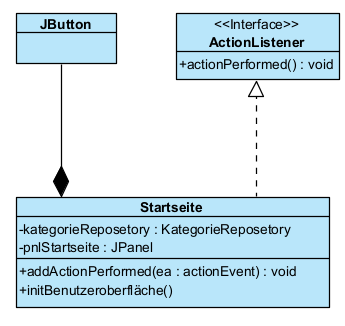
\includegraphics[width=0.70\textwidth]{Bilder/Entwurfsmuster-UML.png} 
	\caption{UML-Diagramm Observer-Pattern Entwurfmuster}
	\label{fig:EntwurfmusterUML}
\end{figure}
\autoref{fig:EntwurfmusterUML} ist das UML-Diagramm unseres Observers am Beispiel der \href{https://github.com/MichaelaHaag/RezeptApp/blob/main/0-Plugins/src/main/java/de/rezeptapp/plugins/gui/Startseite.java}{\code{GUI Startseite}}. 
Auf Grund der Übersichtlichkeit wurden nur die Methoden der Klassen EventListenerList und AbstractButton dargestellt, die für ein besseres Verständnis der Zusammenhänge notwendig sind. 

Der ActionListener in Java hat einige Limitationen. Eine Limitation ist, dass der ActionListener nur für eine Aktion auf einem bestimmten Komponenten-Objekt registriert werden kann, wie z.B. das Klicken auf eine Schaltfläche. Außerdem kann der ActionListener keine Werte zurückgeben, was bedeutet, dass er keine Möglichkeit hat, Feedback oder Informationen an den Aufrufer zurückzugeben, da die Methode actionPerformed vom Typ void ist. Daher kann der ActionListener auch keine Exceptions werfen.
Eine weitere Limitation ist, dass der ActionListener asynchron ausgeführt wird. Er blockiert, bis die Aktion abgeschlossen ist.
Des Weiteren ist ActionListener nur für Mausereignisse geeignet und kann nicht für Tastatureingaben verwendet werden. Dazu kommt, dass der ActionListener nur auf ein einzelnes Mausereignis reagieren kann, wie das Klicken auf eine Schaltfläche oder ein Menüelement. Andere Mausereignisse wie das Bewegen der Maus oder das Drücken der rechten Maustaste werden vom ActionListener nicht akzeptiert. Unser Code arbeitet innerhalb der Limitationen, daher ist der ActionListener für unsere Anwendung gut geeignet. 